\documentclass[utf8x,xcolor=pdftex,dvipsnames,table]{beamer}
\usetheme{Malmoe}  % Now it's a beamer presentation with the lisa theme!
\setbeamertemplate{footline}[page number]
\usecolortheme{beaver}
\usepackage[T1]{fontenc}
\usepackage{amsmath}
\usepackage[utf8x]{inputenc}
\usepackage{listings}

\newcommand{\superscript}[1]{\ensuremath{^{\textrm{#1}}}}

\mode<presentation>

\title{Debugging}

\author{%
\footnotesize
Frédéric Bastien \newline
\newline
\newline
Institut des algorithmes d'apprentissage de Montréal \newline
Montreal Institute for Learning Algorithms \newline
Université de Montréal
}

\date{August 10th, Deep Learning Summer School 2015, Montréal}

\setbeamertemplate{navigation symbols}{}
\begin{document}

\begin{frame}[plain]
 \titlepage
 \vspace{-2em}
 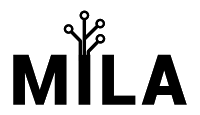
\includegraphics[width=.8in]{mila.png}
 \hfill
 
\includegraphics[width=.8in]{UdeM_logo}
\end{frame}

\section{Introduction}
\begin{frame}{Slides and Exercices}
  \url{http://github.com/mila-udem/summerschool2015/debug}
\end{frame}

\section{Debugging}
\begin{frame}
  \tableofcontents[currentsection]
\end{frame}


\begin{frame}[fragile]
  \frametitle{Error message}
  \begin{itemize}
  \item Very important
  \item Much information in them
  \item Take the time to read them
  \end{itemize}
An Error message have 4 parts:
  \begin{itemize}
  \item The stack trace
  \item The error itself (THE MOST IMPORTANT PART!)
  \item Details about the error message
  \item Sometimes, some HINTs at the end.
  \end{itemize}

  If multiple errors, check the first one.
\end{frame}

\subsection{Error message}
\begin{frame}[fragile]
  \frametitle{Error message: code}
\lstset{language=Python,
        commentstyle=\itshape\color{blue},
        stringstyle=\color{violet},
        }
\begin{lstlisting}
import numpy as np
import theano
import theano.tensor as T
x = T.vector()
y = T.vector()
z = x + x
z = z * y
f = theano.function([x, y], z)
f(np.ones((2,)), np.ones((3,)))
\end{lstlisting}
\end{frame}

\begin{frame}[fragile]
  \frametitle{Error message: 1st part}

\lstset{language=Python,
        commentstyle=\itshape\color{blue},
        stringstyle=\color{violet},
        basicstyle=\scriptsize
        }
\begin{lstlisting}
Traceback (most recent call last):
[...]
ValueError: Input dimension mis-match.
    (input[0].shape[0] = 2, input[1].shape[0] = 3)
Apply node that caused the error:
     Elemwise{Composite{((i0 + i0) * i1)}}(
         <TensorType(float64, vector)>,
         <TensorType(float64, vector)>)
Toposort index: 0
Inputs types: [TensorType(float64, vector),
               TensorType(float64, vector)]
Inputs shapes: [(2,), (3,)]
Inputs strides: [(8,), (8,)]
Inputs values: [array([ 1.,  1.]), array([ 1.,  1.,  1.])]
Outputs clients: [['output']]
\end{lstlisting}
\end{frame}

\begin{frame}[fragile]
  \frametitle{Error message: 2st part}
HINT: Re-running with most Theano optimization
disabled could give you a backtrace when this
node was created. This can be done with by setting
the Theano flags ``optimizer=fast\_compile''. If that does not
work, Theano optimizations can be disabled with
``optimizer=None''.\newline
HINT: Use the Theano flag ``exception\_verbosity=high''
for a debugprint of this apply node.
\end{frame}


\begin{frame}[fragile]
  \frametitle{Error message: Traceback}

\lstset{language=Python,
        commentstyle=\itshape\color{blue},
        stringstyle=\color{violet},
        basicstyle=\footnotesize,
        xleftmargin=-1em
        }
\begin{lstlisting}
Traceback (most recent call last):
  File "test.py", line 9, in <module>
    f(np.ones((2,)), np.ones((3,)))
  File "/u/bastienf/repos/theano/compile/function_module.py",
       line 589, in __call__
    self.fn.thunks[self.fn.position_of_error])
  File "/u/bastienf/repos/theano/compile/function_module.py",
       line 579, in __call__
    outputs = self.fn()
\end{lstlisting}
\end{frame}


\begin{frame}[fragile]
  \frametitle{Error message: optimizer=fast\_compile}

\lstset{language=Python,
        commentstyle=\itshape\color{blue},
        stringstyle=\color{violet},
        }
\begin{lstlisting}
Backtrace when the node is created:
  File "test.py", line 7, in <module>
    z = z * y

\end{lstlisting}
\end{frame}

\subsection{DebugMode}
\begin{frame}[fragile]
  \frametitle{DebugMode}
    Checks and double-checks everything, extremely slow
\begin{itemize}
\item Compare Python, C and GPU implementations.
\item Compare before and after each optimization.
\item By default, raise an error on NaN.
\item Sensitive: so frequently reported errors are ok.
\end{itemize}
\end{frame}

\subsection{Breakpoint}
\begin{frame}[fragile]
  \frametitle{Breakpoint Op} Identity-like op with the side effect of
  enforcing a conditional breakpoint in Python Debugger (PDB), inside a theano function, based
  on a symbolic scalar condition.
\end{frame}

\begin{frame}[fragile]
  \frametitle{Breakpoint Op: optimization}
 Most Theano optimizations don't recognize it except one
 optimization that transfer it to the GPU.
\begin{itemize}
  \item Could slow down computation, but not too much.
  \item Could prevent stability optimizations.
  \item Can be moved to the GPU. It does not add extra transfers.
  \item The output of the breakpoint op must be used in the graph.
\end{itemize}
\end{frame}

\begin{frame}[fragile]
  \frametitle{Breakpoint Op: example}
\lstset{language=Python,
        commentstyle=\itshape\color{blue},
        stringstyle=\color{violet},
        basicstyle=\footnotesize,
        xleftmargin=-1em
        }
\begin{lstlisting}
import theano
import theano.tensor as T
from theano.tests.breakpoint import PdbBreakpoint
input, target = T.fvectors('xy')

mse = (input - target) ** 2

# Conditional breakpoint to be activated if the total
# MSE > 100. The breakpoint will monitor the inputs,
# targets as well as the individual error values
breakpointOp = PdbBreakpoint(``MSE too high'')
condition = T.gt(mse.sum(), 100)
mse, monitored_input, monitored_target = breakpointOp(
    condition, mse, input, target)
\end{lstlisting}
\end{frame}

\begin{frame}[fragile]
  \frametitle{Breakpoint Op: example}
\lstset{language=Python,
        commentstyle=\itshape\color{blue},
        stringstyle=\color{violet},
        basicstyle=\footnotesize,
        xleftmargin=-1em
        }
\begin{lstlisting}
# Compile the theano function
fct = theano.function([input, target], mse)

# Use the function
print fct([10, 0], [10, 5]) # Will NOT activate the breakpoint
print fct([0, 0], [10, 5]) # Will activate the breakpoint
\end{lstlisting}

\end{frame}

\subsection{PrintOp}
\begin{frame}[fragile]
  \frametitle{PrintOp}
Allow to print during execution. The output of the print op must be
used in the graph.
 \vspace{1cm}
\lstset{language=Python,
        commentstyle=\itshape\color{blue},
        stringstyle=\color{violet},
        basicstyle=\footnotesize,
        xleftmargin=-1em
        }
\begin{lstlisting}
import theano
x = theano.tensor.vector()
o = theano.printing.Print(``a message'')(x)
f = theano.function([x], o)
d = f([3, 4])
a message  __str__ = [ 3.  4.]
\end{lstlisting}
\end{frame}


\subsection{Nan}
\begin{frame}
  \frametitle{Most Frequent NaN Causes}
\begin{itemize}
\item Hyperparameters (ex: learning rate)
\item Initialization of parameters
\item Numerical Stability
\item Algorithm Related
\end{itemize}
Run in NanGuardMode, DebugMode, or MonitorMode
\end{frame}

\begin{frame}[fragile]
  \frametitle{NanGuardMode}
\lstset{language=Python,
        commentstyle=\itshape\color{blue},
        stringstyle=\color{violet},
        basicstyle=\footnotesize,
        xleftmargin=-1em
        }
Can check:
\begin{itemize}
\item Nan
\item Inf
\item Big value (greater than 1e10)
\end{itemize}
\end{frame}

\begin{frame}[fragile]
  \frametitle{NanGuardMode: example}
\lstset{language=Python,
        commentstyle=\itshape\color{blue},
        stringstyle=\color{violet},
        basicstyle=\footnotesize,
        xleftmargin=-1em
        }
\begin{lstlisting}
x = T.dmatrix()
w = theano.shared(numpy.random.randn(5, 7))
y = T.dot(x, w)
mode=NanGuardMode(nan_is_error=True,
                  inf_is_error=True,
                  big_is_error=True)
fun = theano.function(
    [x], y, mode=mode)
infa = numpy.tile(
    (numpy.asarray(100.) ** 1000000), (3, 5))
fun(infa)
\end{lstlisting}
\end{frame}

\subsection{Test Value}
\begin{frame}[fragile]
  \frametitle{Test Value}

Give a sample value to symbolic variables and have the graph execution
when you build it. This allow to get some type of error like shape
errors when you build the graph.
 \vspace{1cm}
\end{frame}

\begin{frame}[fragile]
  \frametitle{Test Value: Example}
\lstset{language=Python,
        commentstyle=\itshape\color{blue},
        stringstyle=\color{violet},
        basicstyle=\footnotesize,
        xleftmargin=-1em
        }
\begin{lstlisting}
# Can also be 'off', 'ignore', 'raise', 'pdb'
theano.config.compute_test_value = 'warn'
# input which will be of shape (5, 10)
x, y  = T.matrices('xy')
# provide Theano with a default test-value
x.tag.test_value = numpy.random.rand(5, 10)
y.tag.test_value = numpy.random.rand(4, 10)
x + y # warn about the shape error
\end{lstlisting}

\end{frame}

\subsection{Others}
\begin{frame}
  \frametitle{Others}
  \begin{itemize}
  \item theano.tensor.opt.AssertOp
    \begin{itemize}
    \item Assertion during execution
    \end{itemize}
  \item theano.printing.\{debugprint,pydotprint\}
    \begin{itemize}
    \item Text and graphique display of Theano graph
    \end{itemize}
  \item Flag: profile=True
    \begin{itemize}
    \item Profile the execution time of Theano function
    \end{itemize}
  \item Flag: exception\_verbosity=True
    \begin{itemize}
    \item Extra verbose error, ex: for Memory Error
    \end{itemize}
  \item Flag: warn\_float64='pdb'
    \begin{itemize}
    \item  Allow to know where float64 are build in the graph
    \end{itemize}
  \end{itemize}
\end{frame}

\begin{frame}
  \frametitle{Others: advanced}
  \begin{itemize}
  \item Flag: on\_opt\_err=True
    \begin{itemize}
    \item Make Theano stop of optimization error instead of skipping them
    \end{itemize}
  \item Flag: optimizer\_verbose=True
    \begin{itemize}
    \item Make Theano print each optimization it apply
    \end{itemize}
  \end{itemize}
\end{frame}

\section{Python Debugger (PDB)}
\subsection{Introduction}
\begin{frame}
  \frametitle{Introduction}
  \begin{itemize}
  \item PDB is similar to GDB
  \item 'n': next, 'c': continue, 'l': list, 'p var': print, 's': step, ...
  \item It only check the first letter, don't forget the 'p'!
  \end{itemize}
\end{frame}

\subsection{Theano}
\begin{frame}
  \frametitle{Theano + PDB}
  Can be used with Theano:
  \begin{itemize}
    \item mode=FAST\_COMPILE \# Disable most of opt + c code.
    \item linker=py \# Disable c code.
    \item PdbBreakpoint \# Breakpoing during execution.
    \item Some Theano flags have a pdb value (ex: warn\_float64)
  \end{itemize}
\end{frame}

\begin{frame}{Connection instructions}
\begin{itemize}
\item Navigate to \url{nvlabs.qwiklab.com}
\item Login or create a new account
\item Select the ``Instructor-Led Hands-on Labs'' class
\item Find the lab called ``Theano'' and click Start
\item After a short wait, lab instance connection information will be shown
\item Please ask Lab Assistants for help!
\end{itemize}
\end{frame}

\begin{frame}{Questions, Acknowledgments}
\Huge
\begin{center}
Questions?\newline
Acknowledgments
\end{center}
\normalsize
\begin{itemize}
\item All people working or having worked at the LISA lab/MILA institute
\item All Theano users/contributors
\item Compute Canada, RQCHP, NSERC, and Canada Research Chairs for providing funds or access to compute resources.
\end{itemize}

\end{frame}


\end{document}
